\RequirePackage{plautopatch}
\documentclass[uplatex,dvipdfmx,a4paper,11pt]{jsreport}

\usepackage{docmute}


% 数式
\usepackage{amsmath,amsthm,amssymb}
\usepackage{bm}
% 画像
\usepackage{graphicx}

\usepackage{multirow}
\usepackage{wrapfig}
\usepackage{ascmac}
\usepackage{xcolor}


\usepackage{makeidx}
\makeindex

\graphicspath{{../../_Figures//}{../../_Figures/Rheology/}}

\usepackage{qrcode}
\setlength\lineskiplimit{0pt}
\setlength\normallineskiplimit{0pt}

\usepackage{qexam}

\usepackage{titlesec}
\titleformat*{\section}{\Large\bfseries}
\titleformat*{\subsection}{\large\bfseries}
\titleformat*{\subsubsection}{\normalsize\bfseries}
\titleformat*{\paragraph}{\normalsize\bfseries}

% ページ設定
% \pagestyle{empty}
% 高さの設定
\setlength{\textheight}{\paperheight}   % ひとまず紙面を本文領域に
\setlength{\topmargin}{-5.4truemm}      % 上の余白を20mm(=1inch-5.4mm)に
\addtolength{\topmargin}{-\headheight}  % 
\addtolength{\topmargin}{-\headsep}     % ヘッダの分だけ本文領域を移動させる
\addtolength{\textheight}{-40truemm}    % 下の余白も20mmに%% 幅の設定
\setlength{\textwidth}{\paperwidth}     % ひとまず紙面を本文領域に
\setlength{\oddsidemargin}{-5.4truemm}  % 左の余白を20mm(=1inch-5.4mm)に
\setlength{\evensidemargin}{-5.4truemm} % 
\addtolength{\textwidth}{-40truemm}     % 右の余白も20mmに
% 図と本文との間
%\abovecaptionskip=-5pt
%\belowcaptionskip=-5pt
%
% 全体の行間調整
% \renewcommand{\baselinestretch}{1.0} 
% 図と表
%\renewcommand{\figurename}{Fig.}
%\renewcommand{\tablename}{Tab.}
%

% \makeatletter 
% \def\section{\@startsection {section}{1}{\z@}{1.5 ex plus 2ex minus -.2ex}{0.5 ex plus .2ex}{\large\bf}}
% \def\subsection{\@startsection{subsection}{2}{\z@}{0.2\Cvs \@plus.5\Cdp \@minus.2\Cdp}{0.1\Cvs \@plus.3\Cdp}{\reset@font\normalsize\bfseries}}
% \makeatother 

\usepackage[dvipdfmx,%
 bookmarks=true,%
 bookmarksnumbered=true,%
 colorlinks=false,%
 setpagesize=false,%
 pdftitle={数式に頼らない直感的理解による材料設計のためのレオロジー⼊⾨},%
 pdfauthor={佐々木裕},%
 pdfsubject={},%
 pdfkeywords={レオロジー; 材料設計; }]{hyperref}
\usepackage{pxjahyper}

\usepackage{plext}

\usepackage{niceframe} 
\usepackage{framed}
\newenvironment{longartdeco}{%
  \def\FrameCommand{\fboxsep=\FrameSep \artdecoframe}%
  \MakeFramed {\FrameRestore}}%
 {\endMakeFramed}
 
\usepackage{siunitx}

\newcommand{\rmd}{\mathrm{d}}

\renewcommand{\questionFormat}[1]{
  \begin{center}{\textbf{\large{#1}}}\end{center}
}

\title{第2講 物質のレオロジーに進む前に\\演習問題(解答)}
\author{}
\date{}

\pagestyle{empty}

\begin{document}

\maketitle

\section*{第一章 「物質の物理を理解するために」について (本文 $2\sim18$ p)}
\documentclass[uplatex,dvipdfmx,a4paper,11pt]{jsarticle}

\usepackage{docmute}


% 数式
\usepackage{amsmath,amsthm,amssymb}
\usepackage{bm}
% 画像
\usepackage{graphicx}

\usepackage{multirow}
\usepackage{wrapfig}
\usepackage{ascmac}
\usepackage{xcolor}


\usepackage{makeidx}
\makeindex

\graphicspath{{../../_Figures//}{../../_Figures/Rheology/}}

\usepackage{qrcode}
\setlength\lineskiplimit{0pt}
\setlength\normallineskiplimit{0pt}

\usepackage{qexam}

\usepackage{titlesec}
\titleformat*{\section}{\Large\bfseries}
\titleformat*{\subsection}{\large\bfseries}
\titleformat*{\subsubsection}{\normalsize\bfseries}
\titleformat*{\paragraph}{\normalsize\bfseries}

% ページ設定
% \pagestyle{empty}
% 高さの設定
\setlength{\textheight}{\paperheight}   % ひとまず紙面を本文領域に
\setlength{\topmargin}{-5.4truemm}      % 上の余白を20mm(=1inch-5.4mm)に
\addtolength{\topmargin}{-\headheight}  % 
\addtolength{\topmargin}{-\headsep}     % ヘッダの分だけ本文領域を移動させる
\addtolength{\textheight}{-40truemm}    % 下の余白も20mmに%% 幅の設定
\setlength{\textwidth}{\paperwidth}     % ひとまず紙面を本文領域に
\setlength{\oddsidemargin}{-5.4truemm}  % 左の余白を20mm(=1inch-5.4mm)に
\setlength{\evensidemargin}{-5.4truemm} % 
\addtolength{\textwidth}{-40truemm}     % 右の余白も20mmに
% 図と本文との間
%\abovecaptionskip=-5pt
%\belowcaptionskip=-5pt
%
% 全体の行間調整
% \renewcommand{\baselinestretch}{1.0} 
% 図と表
%\renewcommand{\figurename}{Fig.}
%\renewcommand{\tablename}{Tab.}
%

% \makeatletter 
% \def\section{\@startsection {section}{1}{\z@}{1.5 ex plus 2ex minus -.2ex}{0.5 ex plus .2ex}{\large\bf}}
% \def\subsection{\@startsection{subsection}{2}{\z@}{0.2\Cvs \@plus.5\Cdp \@minus.2\Cdp}{0.1\Cvs \@plus.3\Cdp}{\reset@font\normalsize\bfseries}}
% \makeatother 

\usepackage[dvipdfmx,%
 bookmarks=true,%
 bookmarksnumbered=true,%
 colorlinks=false,%
 setpagesize=false,%
 pdftitle={数式に頼らない直感的理解による材料設計のためのレオロジー⼊⾨},%
 pdfauthor={佐々木裕},%
 pdfsubject={},%
 pdfkeywords={レオロジー; 材料設計; }]{hyperref}
\usepackage{pxjahyper}

\usepackage{plext}

\usepackage{niceframe} 
\usepackage{framed}
\newenvironment{longartdeco}{%
  \def\FrameCommand{\fboxsep=\FrameSep \artdecoframe}%
  \MakeFramed {\FrameRestore}}%
 {\endMakeFramed}
 
\usepackage{siunitx}

\newcommand{\rmd}{\mathrm{d}}

\usepackage[inline]{showlabels}

\begin{document}

\question{演習問題 1}
内容を振り返るために、以下に示した文章例の中から適切な記述のものを複数選んでください。
\begin{qlist}
	\qitem 指数関数と対数関数についての、正しい言葉はどれでしょうか?
		\begin{qlist2}
			\qitem 指数関数とは、「底」と呼ばれる正の数の右肩に「指数」と呼ばれる数を載せた数式表現です。
			\qitem 対数関数とは、指数関数の逆関数になっています。
			\qitem 対数関数は、指数関数に反比例します。
			\qitem 片対数グラフは、指数関数の指数を定めるときに便利に使えます。
			\qitem 指数関数の指数が負の場合($f(x)=\exp(-x)$)、関数 $f(x)$ は単調増加します。
		\end{qlist2}
        \vspace{3mm}
        \begin{itembox}[l]{解答}
            正しい選択肢:(a), (b), (d)\\
            (解説)
			\begin{itemize}
				\item 指数関数の指数が負の場合がレオロジーでよく使われています。
				\item このとき、関数 $f(x)$ は単調減少して 0 に漸近していきますが、決して負にはなりません。
			\end{itemize}
        \end{itembox}
	\qitem 微積分についての、正しい言葉はどれでしょうか?
		\begin{qlist2}
			\qitem 微分は、対象とする関数が注目したい点の周りでどのように振る舞うのかを明らかにします。
			\qitem 微分とは、「分母である変数の変化」と「分子となっている関数の変化」の関係を全体的に見ます。
			\qitem 不定積分とは、微分するとその関数 f(x) に一致するような原始関数 F(x) を求める操作です。
			\qitem 微分で瞬間の描像を取り出し、積分で全体のふるまいを総量として把握できます。
			\qitem 不定積分により、着目する領域の面積を算出することができます。
		\end{qlist2}
        \vspace{3mm}
        \begin{itembox}[l]{解答}
            正しい選択肢:(a), (c), (d)\\
            (解説)
			\begin{itemize}
				\item 微分とは、注目する点における関数の「局所的な振る舞い」を接線の傾きで表したものであり、「僅かな変化の比」を見ることができます。
				\item 微分で瞬間の振る舞いを取り出すことが出来ますし、積分で全体のふるまいを総量として把握することができると理解すればいいでしょう。
			\end{itemize}
        \end{itembox}
	\qitem 微分方程式についての、正しい言葉はどれでしょうか?
		\begin{qlist2}
			\qitem 微分方程式とは、「物理現象や化学現象を、微分の形で記述したもの」です。
			\qitem 微分方程式は、微分を繰り返すことで解くことができます。
			\qitem 微分方程式の例として、「放射性物質の崩壊」等の一次反応と呼ばれる化学現象を挙げることができます。
			\qitem 一次反応の解は、単調増加の振る舞いをします。
			\qitem 指数関数的な減少において、初期濃度の $1/e$ になる時間を緩和時間と呼びます。
		\end{qlist2}
        \vspace{3mm}
        \begin{itembox}[l]{解答}
            正しい選択肢:(a), (c), (e)\\
            (解説)
			\begin{itemize}
				\item 微分方程式は、微分の逆操作である積分を用いることで解くことができます。
				\item 微分方程式の例として一次反応と呼ばれる化学現象があり、その解は指数関数的な減少を表します。
			\end{itemize}
        \end{itembox}
	\qitem 「仕事とエネルギー」についての、正しい言葉はどれでしょうか?
		\begin{qlist2}
			\qitem 仕事とは、「質点に力を作用して、移動すること」と一般に定義されています。
			\qitem 物理量として、「仕事 W は、作用させた力 F と移動した距離 s の積」として定義されます。
			\qitem 仕事の組立単位は、ニュートンです。
			\qitem エネルギーは「仕事をする能力」のことであり、仕事とエネルギーの次元は同一です。
			\qitem 物体や空間(場)は、力学的な仕事を受けることでエネルギーが低い状態となります。
		\end{qlist2}
        \vspace{3mm}
        \begin{itembox}[l]{解答}
            正しい選択肢:(a), (b), (d)\\
            (解説)
			\begin{itemize}
				\item 仕事とは、「質点に力を作用して、移動すること」と一般に定義されていて、その組立単位はジュールです。
				\item 物体や空間(場)は、力学的な仕事を受けることでエネルギーが高い状態となります。
			\end{itemize}
        \end{itembox}
	\qitem 「ポテンシャルと摩擦力」についての、正しい言葉はどれでしょうか?
		\begin{qlist2}
			\qitem ポテンシャルとは、「任意の基準の状態を定めたうえで、着目する状態にするためにその物体あるいは空間に加えた仕事の量」と定義されます。
			\qitem ポテンシャルは、「ある状態から基準の状態に戻るまでに系外から加えなくてはいけないエネルギーの量」と考えることもできます。
			\qitem ポテンシャルは、常に「位置のみの関数として与えられる状態量」ではありません。
			\qitem ポテンシャルを微分すれば力が、力を積分すればポテンシャルが出る表裏一体の関係です。
			\qitem 摩擦を考慮した系においては、保存力ではないのでポテンシャルは定義できません。
		\end{qlist2}
        \vspace{3mm}
        \begin{itembox}[l]{解答}
            正しい選択肢:(a), (d), (e)\\
            (解説)
			\begin{itemize}
				\item ポテンシャルは、「ある状態から基準の状態に戻るまでに外に取り出すことのできるエネルギーの量」と考えることができます。
				\item そして、力が「保存力」であるときだけ「位置のみの関数として与えられる状態量」となります。
				\item 摩擦力は非保存力であるため、摩擦を考慮した系における仕事は経路に依存することになります。
			\end{itemize}
        \end{itembox}
\end{qlist}

\question{演習問題 2}
内容を振り返るために、テキストで用いた言葉を使って簡単な穴埋めを行ってください。
\begin{qlist}
	\qitem 「指数関数と対数関数」について、\qbox{(a)}から\qbox{(i)}までのカッコを埋めてください。
		\begin{qlist2}
			\qitem 指数関数の特徴について。
			\begin{center}
				\begin{minipage}{0.48\textwidth}
					\begin{itembox}[l]{指数関数の特徴}
						\begin{itemize}
							\item \textcolor{red}{$\exp (x)$ は、\qbox{} します。}
							\item \textcolor{green}{$\exp (-x) = \left(\dfrac{1}{e} \right)^x$ は、\\\qbox{} です。}
							\item 常に、点$(0,1)$を通る。
							\item $x$軸($y=0$)を\qbox{}とする。
						\end{itemize}
					\end{itembox}
				\end{minipage}
				\begin{minipage}{0.4\textwidth}
					\begin{center}
					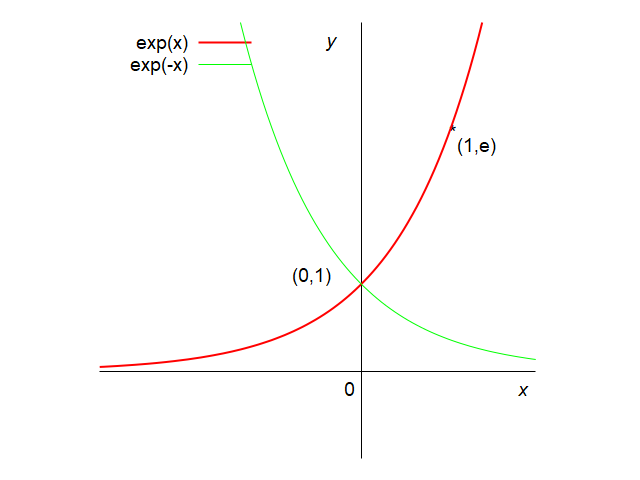
\includegraphics[width=\textwidth]{exp.png}
					\end{center}
				\end{minipage}
			\end{center}
			
			\qitem 指数関数と対数関数。
			\begin{center}
				\begin{minipage}{0.48\textwidth}
					\begin{itembox}[l]{指数関数と対数関数}
						\vspace{-3mm}
						\begin{align*}
							\textcolor{blue}{a}^{\textcolor{red}{x}} = \textcolor{green}{M} \Leftrightarrow \textcolor{red}{x}= \log_{\textcolor{blue}{a}} \textcolor{green}{M}
						\end{align*}
						\begin{itemize}
							\item 指数関数:\\底に\qbox{}を作用させて真数を求める関数
							\item 対数関数:\\真数は\qbox{}にどんな指数を与えたものかを求める関数
							\item \qbox{}に関して対称
						\end{itemize}
					\end{itembox}
				\end{minipage}
				\begin{minipage}{0.4\textwidth}
					\begin{center}
					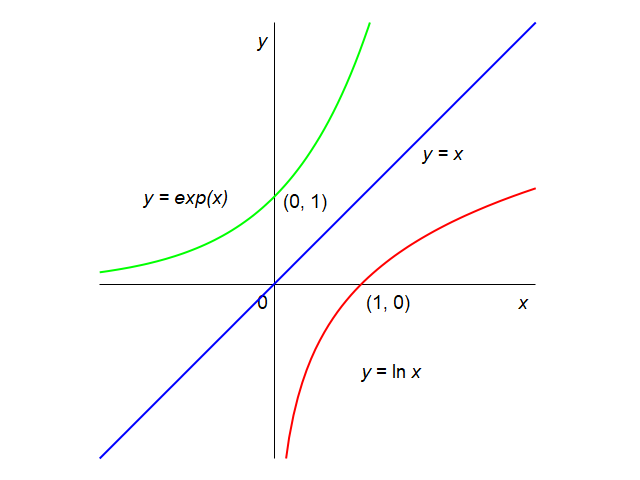
\includegraphics[width=\textwidth]{exp_ln.png}
					\end{center}
				\end{minipage}
			\end{center}

			\qitem 片対数グラフについて。
			\begin{center}
				\begin{minipage}{0.48\textwidth}
					\begin{itembox}[l]{片対数グラフの例}
						\begin{itemize}
							\item 指数関数を取り扱う際に、両辺の対数を取ると、\\
							$\ln y = ax + b$
							\begin{itemize}
								\item 関数値の\qbox{}が、
								\item 変数の\qbox{}となる。
								\item 指数が\qbox{}として求まる。
							\end{itemize}
						\end{itemize}
					\end{itembox}
				\end{minipage}
				\begin{minipage}{0.4\textwidth}
					\begin{center}
					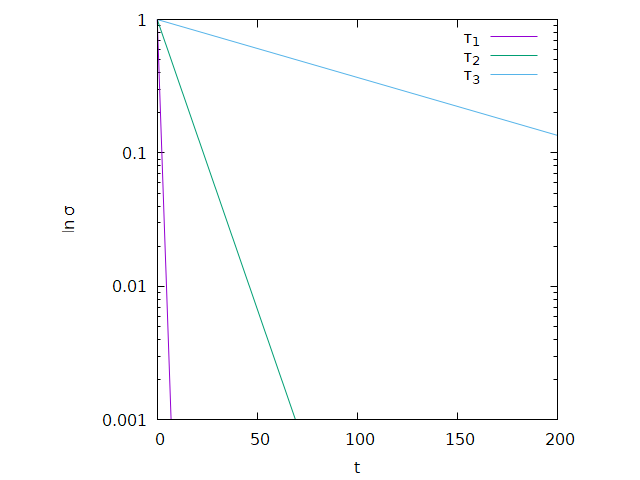
\includegraphics[width=\textwidth]{relux_6.png}
					\end{center}
				\end{minipage}
			\end{center}
		\end{qlist2}

		\begin{itembox}[l]{選択肢}
			\begin{center}
				\begin{tabular}{lllll}
					1. 底	&2. 1次関数	&3. 漸近線	&4. $y=x$	&5. 単調減少\\
					6. 指数	&7. 単調増加		&8. 対数				&9. 傾き
				\end{tabular}
			\end{center}
		\end{itembox}
\end{qlist}

\begin{itembox}[l]{解答}
    \begin{center} 
      \begin{tabular}{|c|c|c|c|c|c|c|c|c|} \hline
        (a) & (b) & (c) & (d) & (e) & (f) & (g) & (h) & (i)\\ \hline
        7 & 5 & 3 & 6 & 1 & 4 & 8 & 2 & 9 \\ \hline		
      \end{tabular}
    \end{center}
\end{itembox}

\begin{qlist}
	\qitem 微積分と微分方程式について、以下の\qbox{(j)}から\qbox{(q)}までのカッコを埋めてください。
		\begin{qlist2}
			\qitem 微分の直感的理解
			\begin{center}
				\begin{minipage}{0.48\textwidth}
					\begin{itembox}[l]{微分の直感的説明}
						\begin{itemize}
							\item 注目する点近傍での接線の\qbox{}
							\begin{itemize}
								\item 変数の増分と、
								\item \qbox{}との比をとる。
							\end{itemize}
							\item 変数の増分を\qbox{}にする。
						\end{itemize}
					\end{itembox}
				\end{minipage}
				\begin{minipage}{0.4\textwidth}
					\begin{center}
					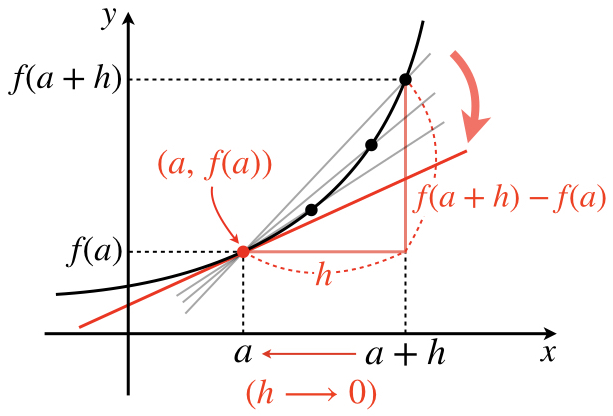
\includegraphics[width=\textwidth]{bibun.jpeg}
					\end{center}
				\end{minipage}
			\end{center}
	\qitem 微分方程式の解き方の例。
		\begin{itembox}[l]{一次反応を表す微分方程式}
			\textbf{1st step: }方程式の両辺に $\rmd t$ を掛ける。
			\begin{align*}
				\dfrac{1}{N} \mathrm{d}N= \qbox{}
			\end{align*}

			\textbf{2nd step: }方程式の両辺に積分記号 $\int$ をつける。
			\begin{align*}
				\int \dfrac{1}{N} \rmd N = \qbox{}
			\end{align*}

			\textbf{3rd step: }両辺の不定積分を計算する。
			\begin{align*}
				\qbox{} = -at + C_2
			\end{align*}

			\textbf{4th step: }積分定数を一つ($C=C_2-C_1$)にまとめる。
			\begin{align*}
				\ln N = -at + C
			\end{align*}

			\textbf{5th step: }指数関数に書き直してから、定数項を書き直し($C'=\exp(C)$)。
			\begin{align*}
				N= \qbox{} = \exp(C) \times \exp(-at) = C' \exp(-at)
			\end{align*}

			\textbf{6th step: }初期条件から、
			\begin{align*}
				&N(t=0) = C' \exp(-a*0) = N_0 \\
				\therefore\; &C' = N_0
			\end{align*}

			\textbf{Final step: }上記の定数項を用いて、濃度は時間の関数として以下となる。
			\begin{align*}
				N(t) = \qbox{}
			\end{align*}
	\end{itembox}
	\end{qlist2}
	\begin{itembox}[l]{選択肢}
		\begin{center}
			\begin{tabular}{llll}
				1. $\exp(-at + C)$	&2. $-a \int \mathrm{d} t$	&3. 無限小	&4. 傾き\\
				5. $\ln N +C_1$ &6. $-a\mathrm{d} t$	&7. 関数の増分	&8 $N_0 \exp(-at)$
			\end{tabular}
		\end{center}
	\end{itembox}
\end{qlist}

\begin{itembox}[l]{解答}
    \begin{center} 
      \begin{tabular}{|c|c|c|c|c|c|c|c|} \hline
        (j) & (k) & (l) & (m) & (n) & (o) & (p) & (q) \\ \hline
        4 & 7 & 3 & 6 & 2 & 5 & 1 & 8 \\ \hline		
      \end{tabular}
    \end{center}
\end{itembox}

\begin{qlist}
	\qitem 力学的な物理量について、以下の\qbox{(r)}から\qbox{(z)}までのカッコを埋めてください。
		\begin{qlist2}
			\qitem 仕事とエネルギーについて
			\begin{center}
				\begin{minipage}{0.42\textwidth}
					\begin{itembox}[l]{仕事とは}
						\begin{itemize}
							\item 質点に力を作用して、移動すること
							\item 仕事は、\qbox{} $F$ と移動した距離 $s$ の積
						\end{itemize}
							
\includegraphics[width=.8\textwidth]{work.png}
					\end{itembox}
				\end{minipage}
				\begin{minipage}{0.42\textwidth}
					\begin{itembox}[l]{エネルギーとは}
						\begin{itemize}
							\item 仕事をする\qbox{}のこと
							\item 物体や空間(場)は、その状態を変えることによりエネルギーを蓄える。
							\item 仕事とエネルギーの\qbox{}は同一。
						\end{itemize}
					\end{itembox}
				\end{minipage}
			\end{center}
			\qitem ポテンシャルについて
				\begin{itembox}[l]{ポテンシャルとは?}
					\begin{itemize}
						\item 基準の状態を定めて、
						\begin{itemize}
							\item 着目する状態にするために、その物体あるいは空間に加えた\qbox{}
						\end{itemize}
						\item 逆に言えば
						\begin{itemize}
							\item ある状態から基準の状態に戻るまでに、外に取り出すことのできる\qbox{}
						\end{itemize}
						\item 力が経路によらない\qbox{}であれば、ポテンシャルが位置のみの関数の状態量となる
					\end{itemize}
				\end{itembox}
			\qitem 摩擦と熱について
			\begin{center}
				\begin{minipage}{0.5\textwidth}
					\begin{itembox}[l]{摩擦と熱}
						\begin{itemize}
							\item 摩擦力は\qbox{}
								% \begin{itemize}
								% 	\item ポテンシャルは状態量ではなく経路に依存
								% \end{itemize}
							\item 内部の粒子の摩擦により、
								\begin{itemize}
									\item 粒子の運動エネルギーが増加し系全体の温度が\qbox{}
									\item 非断熱系では、熱エネルギーとして外界に散逸。
								\end{itemize}
							\item 非保存力も含めれば、系全体のエネルギーは\qbox{}
						\end{itemize}
					\end{itembox}
				\end{minipage}
				\begin{minipage}{0.34\textwidth}
					\begin{center}
					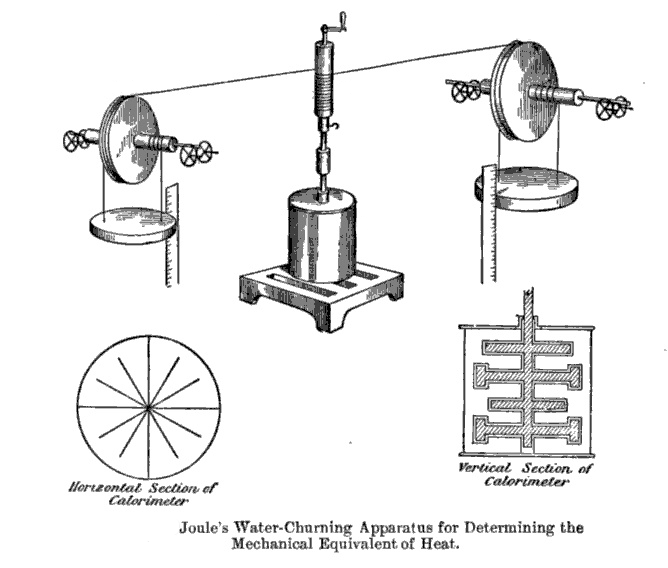
\includegraphics[width=\textwidth]{thermal_eng.png}
					\end{center}
				\end{minipage}
			\end{center}
		\end{qlist2}
	\begin{itembox}[l]{選択肢}
		\begin{center}
			\begin{tabular}{lllll}
				1. 非保存力	&2. 次元	&3. 上昇	&4. 仕事の量 &5. 保存力\\
				6. エネルギーの量	&7. 能力	&8 作用させた力 &9. 保存
			\end{tabular}
		\end{center}
	\end{itembox}
\end{qlist}

\begin{itembox}[l]{解答}
    \begin{center} 
      \begin{tabular}{|c|c|c|c|c|c|c|c|c|} \hline
        (r) & (s) & (t) & (u) & (v) & (w) & (x) & (y) & (z) \\ \hline
        8 & 7 & 2 & 4 & 6 & 5 & 1 & 3 & 9 \\ \hline		
      \end{tabular}
    \end{center}
\end{itembox}

\end{document}
\clearpage

\clearpage
\section*{第二章 「物理化学として物質を見直すと」について (本文 $20\sim35$ p)}
\documentclass[uplatex,dvipdfmx,a4paper,11pt]{jsarticle}

\usepackage{docmute}


% 数式
\usepackage{amsmath,amsthm,amssymb}
\usepackage{bm}
% 画像
\usepackage{graphicx}

\usepackage{multirow}
\usepackage{wrapfig}
\usepackage{ascmac}
\usepackage{xcolor}


\usepackage{makeidx}
\makeindex

\graphicspath{{../../_Figures//}{../../_Figures/Rheology/}}

\usepackage{qrcode}
\setlength\lineskiplimit{0pt}
\setlength\normallineskiplimit{0pt}

\usepackage{qexam}

\usepackage{titlesec}
\titleformat*{\section}{\Large\bfseries}
\titleformat*{\subsection}{\large\bfseries}
\titleformat*{\subsubsection}{\normalsize\bfseries}
\titleformat*{\paragraph}{\normalsize\bfseries}

% ページ設定
% \pagestyle{empty}
% 高さの設定
\setlength{\textheight}{\paperheight}   % ひとまず紙面を本文領域に
\setlength{\topmargin}{-5.4truemm}      % 上の余白を20mm(=1inch-5.4mm)に
\addtolength{\topmargin}{-\headheight}  % 
\addtolength{\topmargin}{-\headsep}     % ヘッダの分だけ本文領域を移動させる
\addtolength{\textheight}{-40truemm}    % 下の余白も20mmに%% 幅の設定
\setlength{\textwidth}{\paperwidth}     % ひとまず紙面を本文領域に
\setlength{\oddsidemargin}{-5.4truemm}  % 左の余白を20mm(=1inch-5.4mm)に
\setlength{\evensidemargin}{-5.4truemm} % 
\addtolength{\textwidth}{-40truemm}     % 右の余白も20mmに
% 図と本文との間
%\abovecaptionskip=-5pt
%\belowcaptionskip=-5pt
%
% 全体の行間調整
% \renewcommand{\baselinestretch}{1.0} 
% 図と表
%\renewcommand{\figurename}{Fig.}
%\renewcommand{\tablename}{Tab.}
%

% \makeatletter 
% \def\section{\@startsection {section}{1}{\z@}{1.5 ex plus 2ex minus -.2ex}{0.5 ex plus .2ex}{\large\bf}}
% \def\subsection{\@startsection{subsection}{2}{\z@}{0.2\Cvs \@plus.5\Cdp \@minus.2\Cdp}{0.1\Cvs \@plus.3\Cdp}{\reset@font\normalsize\bfseries}}
% \makeatother 

\usepackage[dvipdfmx,%
 bookmarks=true,%
 bookmarksnumbered=true,%
 colorlinks=false,%
 setpagesize=false,%
 pdftitle={数式に頼らない直感的理解による材料設計のためのレオロジー⼊⾨},%
 pdfauthor={佐々木裕},%
 pdfsubject={},%
 pdfkeywords={レオロジー; 材料設計; }]{hyperref}
\usepackage{pxjahyper}

\usepackage{plext}

\usepackage{niceframe} 
\usepackage{framed}
\newenvironment{longartdeco}{%
  \def\FrameCommand{\fboxsep=\FrameSep \artdecoframe}%
  \MakeFramed {\FrameRestore}}%
 {\endMakeFramed}
 
\usepackage{siunitx}

\newcommand{\rmd}{\mathrm{d}}

\usepackage[inline]{showlabels}

\begin{document}

\question{演習問題 1}
内容を振り返るために、以下に示した文章例の中から適切な記述のものを複数選んでください。
\begin{qlist}
	\qitem 物質の三態についての、正しい言葉はどれでしょうか?
		\begin{qlist2}
			\qitem マクロな視点で考えると、気体と液体は流れますが、固体は流れなくて形状を変えません。
			\qitem 固体は、何らかの粒子が規則的に並んだ「結晶」としてモデル化される場合が多く見受けられます。
			\qitem 固体の粒子間隔は、一般に液体のそれよりも長くなっています。
			\qitem 液体をミクロに見ても、内部には一見してわかるような規則的な構造を有しません。
			\qitem 気体において粒子は自由に運動していますが、その粒子間隔は液体よりも短くなっています。
		\end{qlist2}
        \vspace{3mm}
        \begin{itembox}[l]{解答}
            正しい選択肢:(a), (b), (d)\\
            (解説)
			\begin{itemize}
				\item 固体のモデルである結晶においては一般に粒子間隔が短く、液体では気体の粒子間隔は長くなっています。
				\item なお、粒子間隔は密度の逆数です。
				\item 液体をミクロに見ても、内部には一見してわかるような規則的な構造を持たないことに注意してください。
			\end{itemize}
        \end{itembox}
	\qitem ミクロに見た場合に粒子間に働く相互作用についての、正しい言葉はどれでしょうか?
		\begin{qlist2}
			\qitem 固体をミクロに見たとき、内部の粒子間に相互作用が存在すると考えられます。
			\qitem Lennard-Jones ポテンシャルは、相対的に速く消失する引力と遠くまで働く斥力との差として二体間の相互作用を表します。
			\qitem ポテンシャルを積分すると働く力が算出できます。
			\qitem ポテンシャルの極小値において二粒子間の力は 0 となります。
			\qitem 粒子間の距離が短くなりすぎると斥力が働き、離れすぎると引力が働きますから、その間に安定状態があります。
		\end{qlist2}
        \vspace{3mm}
        \begin{itembox}[l]{解答}
            正しい選択肢:(a), (d), (e)\\
            (解説)
			\begin{itemize}
				\item Lennard-Jones ポテンシャルは、二体間の相互作用を書き表したポテンシャルです。
				\item これは、相対的に速く消失する斥力に起因するものと遠くまで働く引力によるものとの「和」として表されていることに注意してください。
				\item このポテンシャルを「微分」すると、二体間に働く力が算出できます。
			\end{itemize}
        \end{itembox}
	\qitem 「固体と液体」についての、正しい言葉はどれでしょうか?
		\begin{qlist2}
			\qitem 固体と液体との境目で融解や結晶化が生じるとき、比熱や体積は連続的に変化します。
			\qitem 固体の融解や液体の結晶化において、物質の内部で粒子のパッキングや運動状態も変化します。
			\qitem 液体を形成する粒子の相互の位置は、規則的では有りません。
			\qitem マクロな状態は、ミクロな粒子が熱エネルギーにより自由に動こうとするという状態と居心地のいい位置に留まりたいという状態との2つの状態のせめぎあいで決まります。
			\qitem 液体では、熱の影響が相対的に小さいので、それぞれの粒子が自由に移動します。
		\end{qlist2}	
        \vspace{3mm}
        \begin{itembox}[l]{解答}
            正しい選択肢:(b), (c), (d)\\
            (解説)
            \begin{itemize}
				\item 固体と液体との境目で融解や結晶化が生じるときには比熱や体積に「飛び」が生じます。
				\item このとき、物質の内部では粒子のパッキングや運動状態も変化していると考えられています。
				\item マクロな状態はミクロな粒子がどのように運動するかで決まり、これは、熱エネルギーとポテンシャルとの釣り合いで決まります。
				\item 熱の影響が相対的に大きくてそれぞれの粒子が一箇所に留まらない状態が液体です。
			\end{itemize}
        \end{itembox}
	\qitem 流れるということについての、正しい言葉はどれでしょうか?
		\begin{qlist2}
			\qitem 液体が流れるときには、内部の粒子が瞬間ごとの居心地のいい状態に移動しています。
			\qitem 固体と呼ばれるものは、いくら長時間待っていても決して流れません。
			\qitem 液体を速く変形すると固体的に振る舞う場合があります。
			\qitem 液体を冷却すると、結晶化するとは限らないでガラス状態になることもあります。
			\qitem ガラス化するときも、一般には体積に飛びが出てきます。
		\end{qlist2}	
        \vspace{3mm}
        \begin{itembox}[l]{解答}
            正しい選択肢:(a), (c), (d)\\
            (解説)
			\begin{itemize}
				\item 固体と呼ばれるものであっても、非常に長時間観察していると流れる場合もあります。
				\item  一方、液体も固体的に振る舞うこともありますから、その境目は曖昧です。
				\item また、ガラス化してもミクロに内部を見た時には液体と見分けが付きませんから、一般に体積の飛びは有りません。
			\end{itemize}
        \end{itembox}
	\qitem 応力の由来についての、正しい言葉はどれでしょうか?
		\begin{qlist2}
			\qitem 固体の応力は、内部のミクロな粒子が安定な位置から変位した結果生じると考えられます。
			\qitem 固体内部の応力は、変形すれば直ちに消失します。
			\qitem 液体を変形させると、局所的に歪んだかごのような状態ができます。
			\qitem 液体においても、居心地のいい状態からの変位で応力が発生します。
			\qitem 歪んだ液体で生じた局所的な応力は、流れても消えません。
		\end{qlist2}
        \vspace{3mm}
        \begin{itembox}[l]{解答}
            正しい選択肢:(a), (c), (d)\\
            (解説)
			\begin{itemize}
				\item 固体内部で生じる応力はミクロな粒子の変位によるものであり、外部からの変形が維持されていれば、一般には解消されません。
				\item 一方、液体で生じる局所的な応力は、ミクロな粒子の運動によるマクロな流動とともに消失します。
			\end{itemize}
        \end{itembox}
\end{qlist}

\clearpage

\question{演習問題 2}
内容を振り返るために、テキストで用いた言葉を使って簡単な穴埋めを行ってください。
\begin{qlist}
	\qitem 「固体と液体」について、\qbox{(a)}から\qbox{(i)}までのカッコを埋めてください。
		\begin{qlist2}
			\qitem 粒子多体系での相互作用について
				\begin{center}
					\begin{minipage}{0.52\textwidth}
						\begin{itembox}[l]{多体系での相互作用}
							\begin{itemize}
								\item 多体の\qbox{}を簡略化して、
								\item \qbox{}の相互作用に基づくとすれば、
								\item 多体の粒子が\qbox{}の近傍で摂動
							\end{itemize}
						\end{itembox}
					\end{minipage}
					\begin{minipage}{0.32\textwidth}
						\begin{center}
						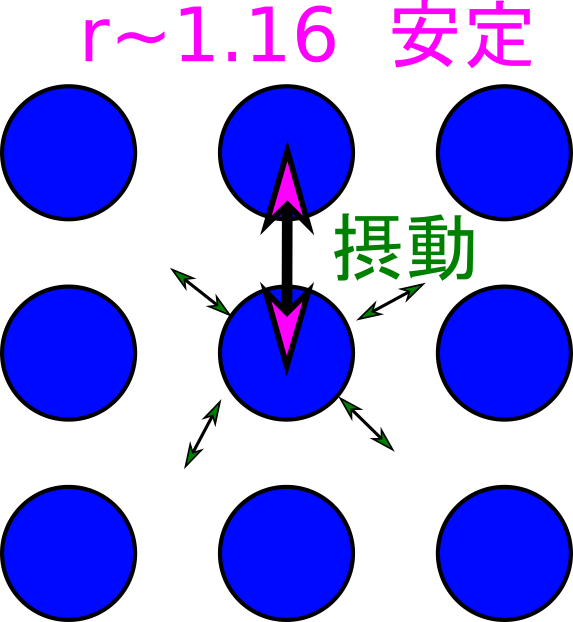
\includegraphics[width=.6\textwidth]{LJ_ryusi.png}
						\end{center}
					\end{minipage}
			\end{center}

		\qitem 固体と液体の相転移について
			\begin{center}
				\begin{minipage}{0.42\textwidth}
					\begin{itembox}[l]{固体と液体の相転移}
						\begin{itemize}
							\item マクロに見れば
							\begin{itemize}
								\item 融解、結晶時に、
								\item \qbox{}に「飛び」
							\end{itemize}
							\item ミクロに考えると、
							\begin{itemize}
								\item 内部の\qbox{}が変化
								\item \qbox{}も変化
							\end{itemize}
						\end{itemize}
					\end{itembox}
				\end{minipage}
				\begin{minipage}{0.42\textwidth}
					\begin{center}
					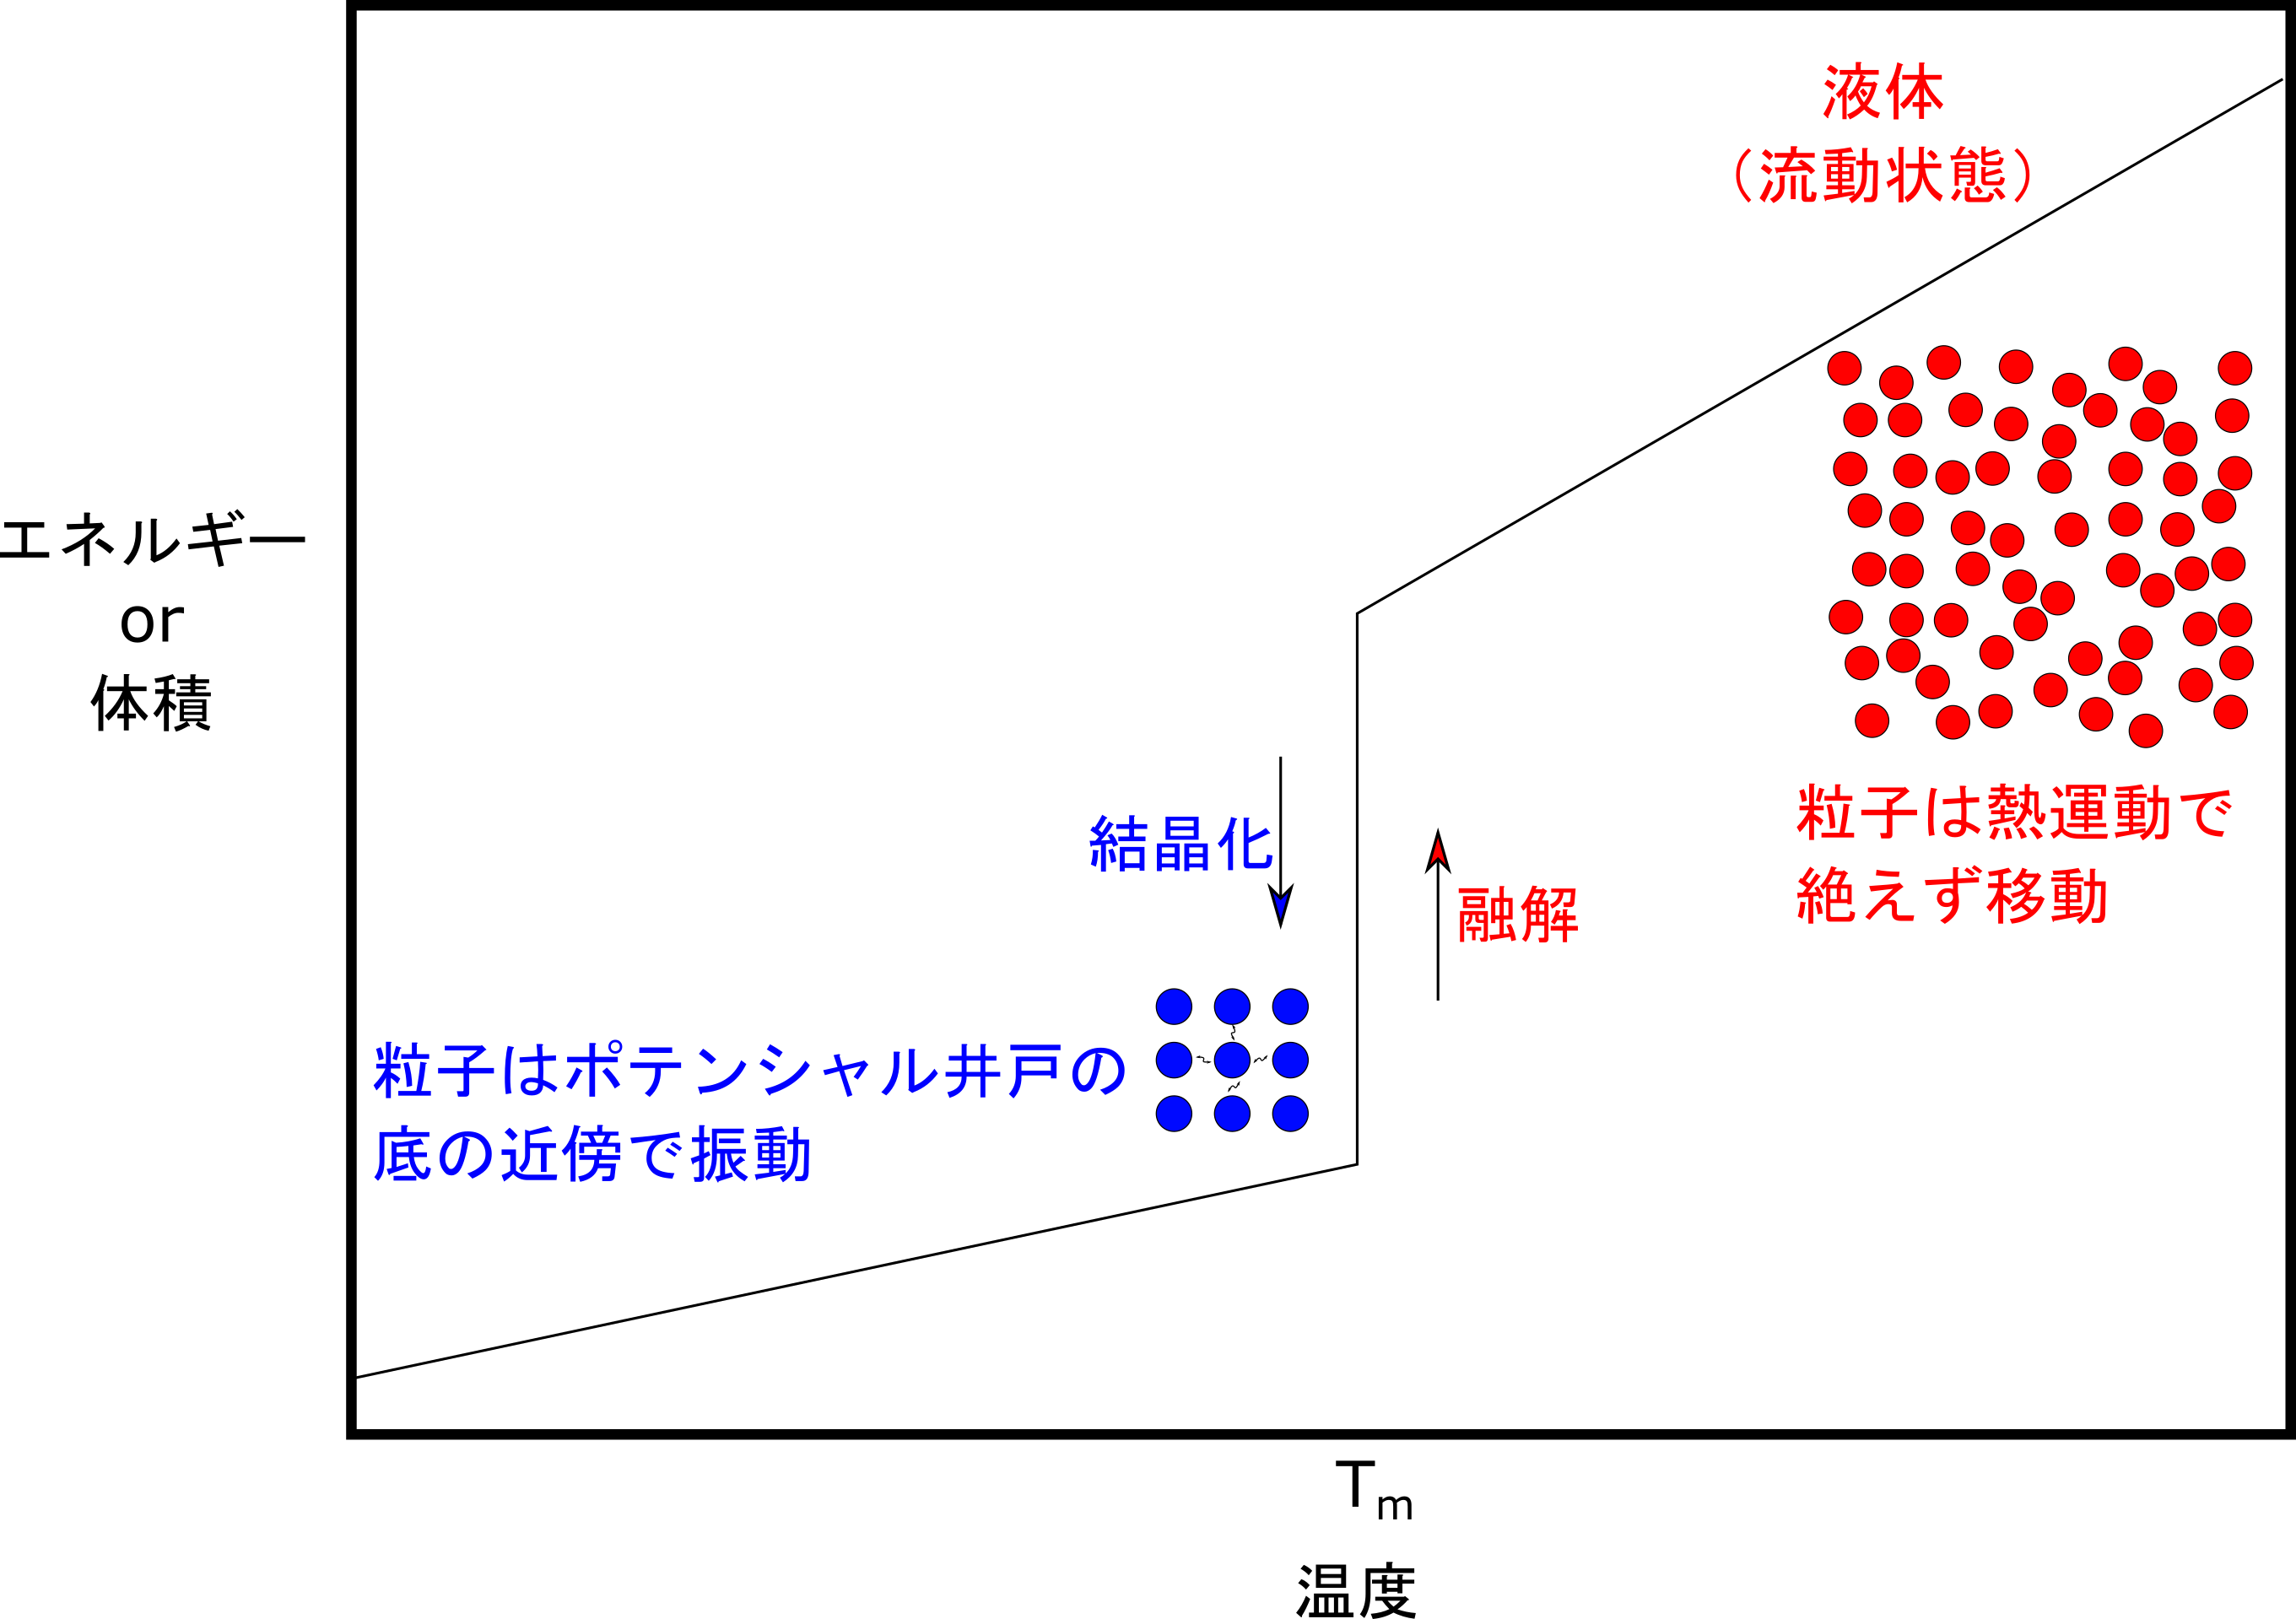
\includegraphics[width=\textwidth]{crystal_melt.png}
					\end{center}
				\end{minipage}
			\end{center}
			
			\qitem 固体と液体の違いとは
				\begin{itembox}[l]{ミクロに考えた固体と液体の違い}
					\begin{itembox}[l]{ミクロな状態での2つのせめぎあい}
						\begin{itemize}
							\item 粒子は\qbox{}で揺らされる。
							\item \qbox{}のいい位置に留まりたい。
						\end{itemize}
					\end{itembox}
					\begin{itembox}[l]{その結果として、}
						\begin{itemize}
							\item 固体:相対的に揺動小
							\begin{itemize}
								\item ポテンシャル井戸の底近傍で振動
								\item 内部構造を形成。
							\end{itemize}
							\item 液体:熱揺動が大きい
							\begin{itemize}
								\item 多くの粒子が相互作用
								\item 構造が\qbox{}
							\end{itemize}
						\end{itemize}
					\end{itembox}
				\end{itembox}

		\end{qlist2}

		\begin{itembox}[l]{選択肢}
			\begin{center}
				\begin{tabular}{lllll}
					1. 熱エネルギー	&2. 相互作用	&3. 居心地	&4. 運動状態	&5. 不定\\
					6. 二体間	&7. 比熱や体積		&8. パッキング	&9. 安定状態
				\end{tabular}
			\end{center}
		\end{itembox}
\end{qlist}

\begin{itembox}[l]{解答}
    \begin{center} 
      \begin{tabular}{|c|c|c|c|c|c|c|c|c|} \hline
        (a) & (b) & (c) & (d) & (e) & (f) & (g) & (h) & (i)\\ \hline
        2 & 6 & 9 & 7 & 4 & 8 & 1 & 3 & 5 \\ \hline		
      \end{tabular}
    \end{center}
\end{itembox}


\begin{qlist}
	\qitem 「流れるということ」について、\qbox{(j)}から\qbox{(r)}までのカッコを埋めてください。
		\begin{qlist2}
			\qitem ミクロに見た流動のイメージ
				\begin{center}
					\begin{minipage}{0.56\textwidth}
						\begin{itembox}[l]{ミクロな流動のイメージ}
							\begin{itemize}
								\item マクロな変形を与える。
								\begin{itemize}
									\item ミクロに粒子の相互位置が変化
									\item 相互のポテンシャルのために、\qbox{}粒子が発生。
									\item 粒子の移動のバランスが変化
									\item 居心地のいい位置へと\qbox{}
								\end{itemize}
								\item マクロな変形に従うように、粒子の位置が\qbox{}。
							\end{itemize}
						\end{itembox}
					\end{minipage}
					\begin{minipage}{0.3\textwidth}
						\begin{center}
						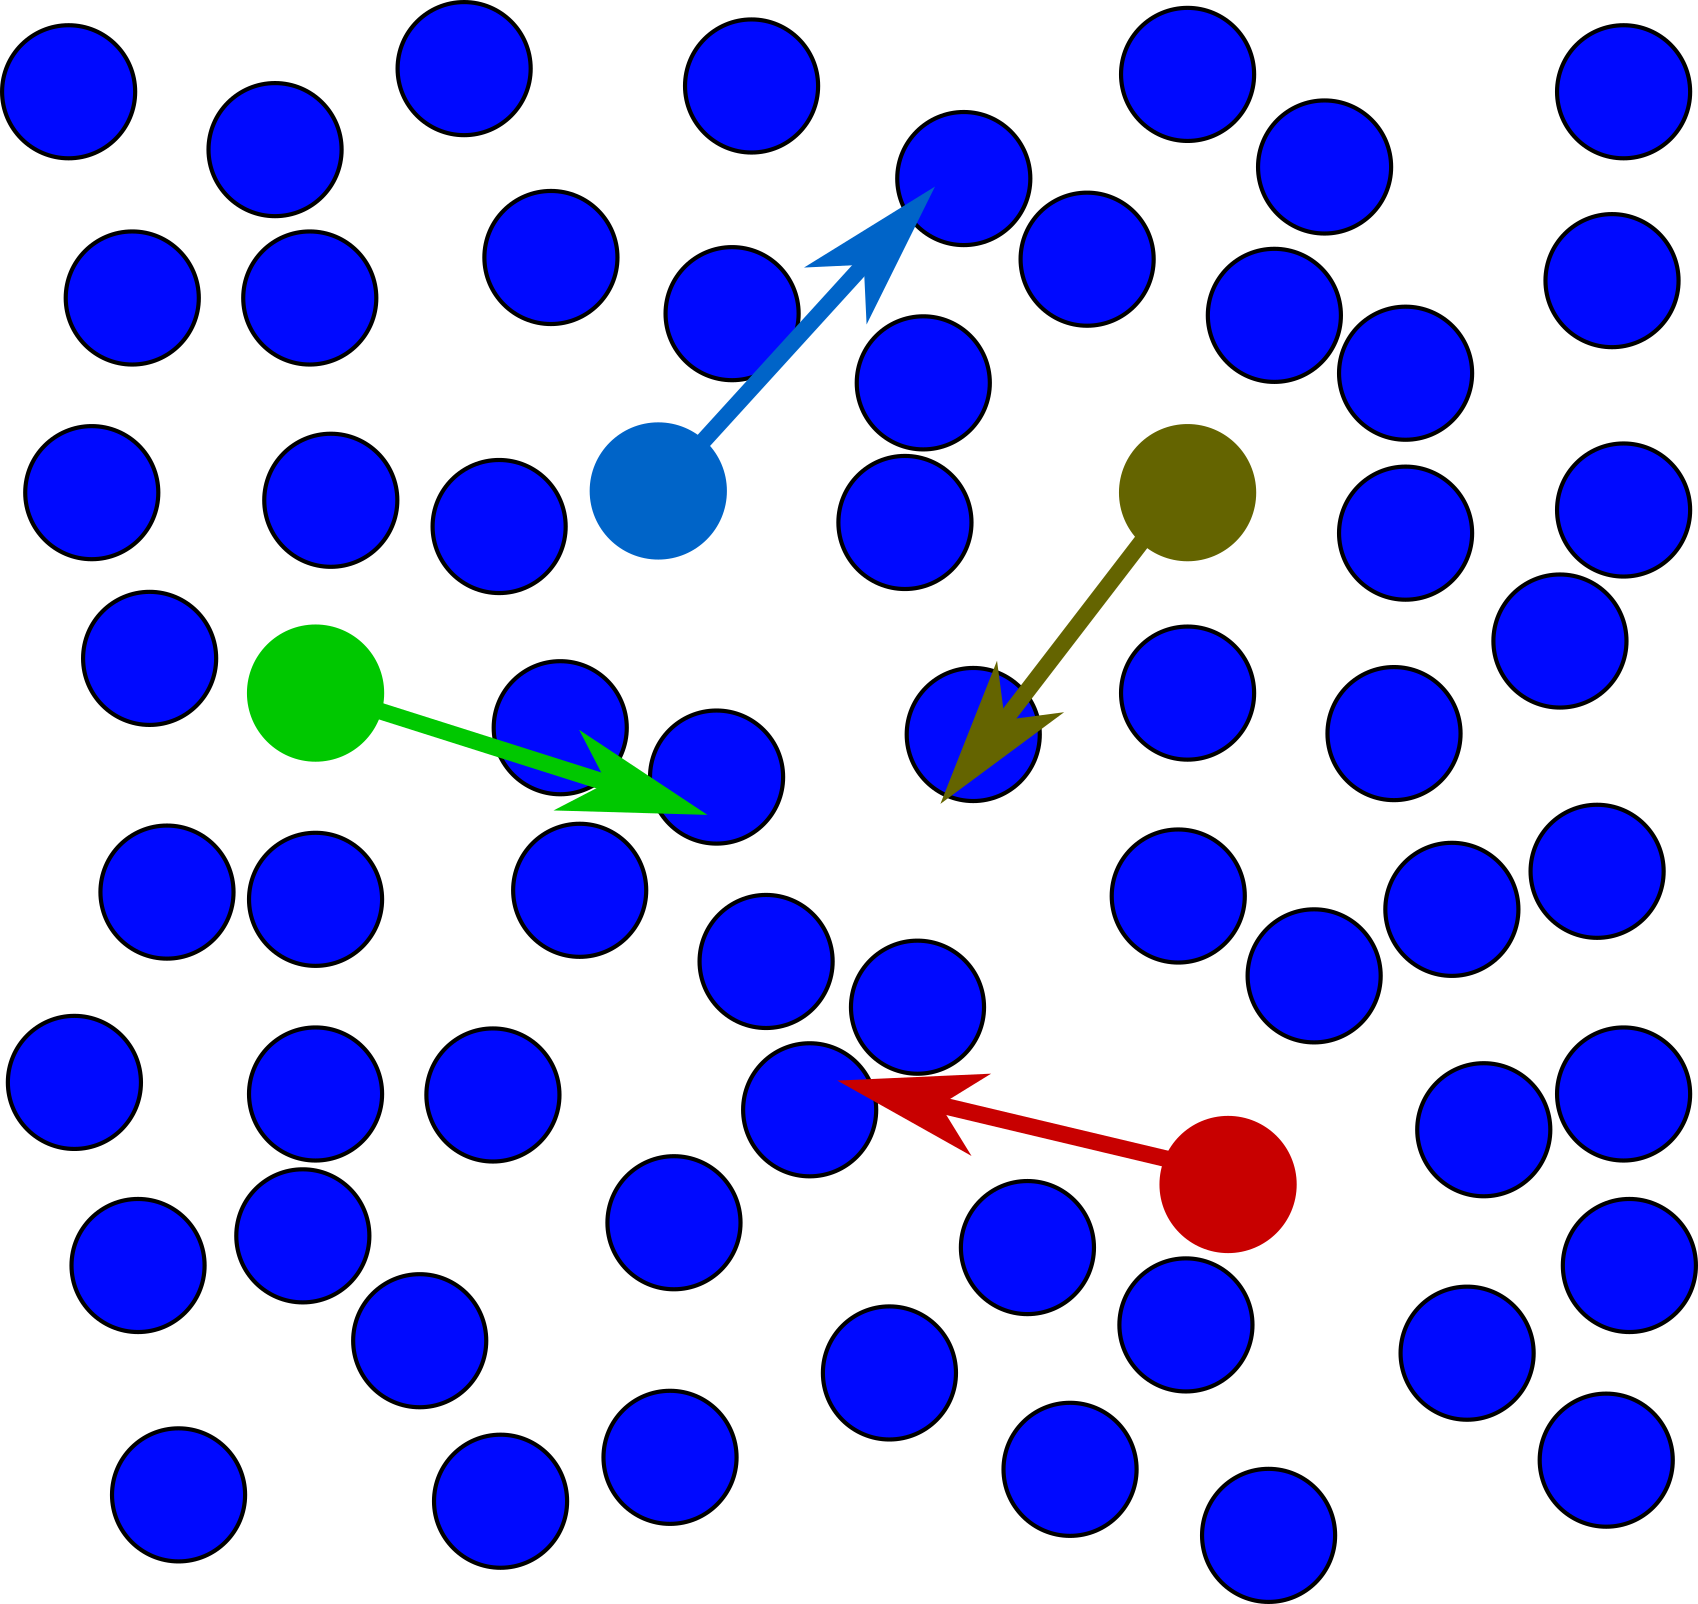
\includegraphics[width=.8\textwidth]{liquid_model_2.png}
						\end{center}
					\end{minipage}
				\end{center}

			\qitem 固体と液体の境目は?
				\begin{center}
					\begin{minipage}{0.44\textwidth}
						\begin{center}
						\begin{itembox}[l]{\qbox{}では固体的に}
							\begin{itemize}
								\item 流動するとは、
								\begin{itemize}
									\item 隙間に粒子が移動
									\item \qbox{}に他の粒子が移動
								\end{itemize}
								\item 粒子が動くより速く変形しようとすると?
								\begin{itemize}
									\item 速い速度で水を変形\\(高所から飛び込み)
									\item 液体が固体的な挙動
								\end{itemize}
							\end{itemize}
						\end{itembox}
						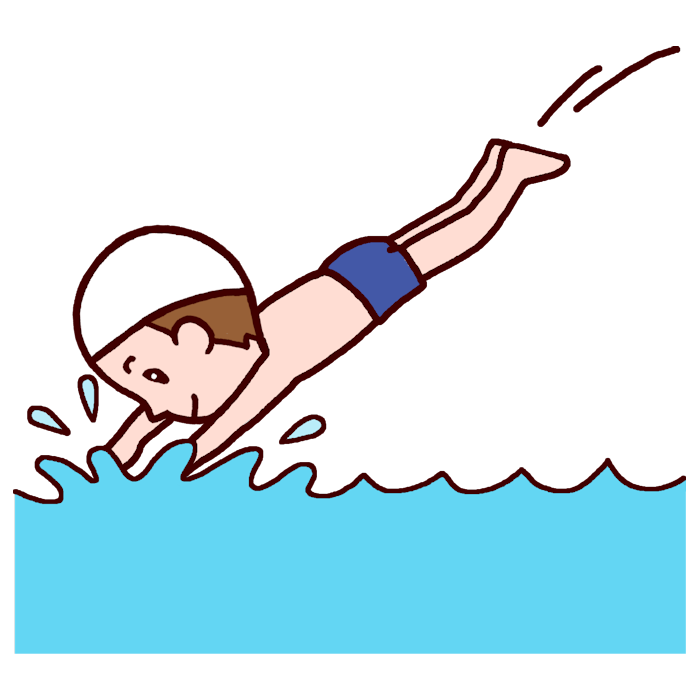
\includegraphics[width=.32\textwidth]{dive.png}
						\end{center}
					\end{minipage}
					\begin{minipage}{0.42\textwidth}
						\begin{center}
						\begin{itembox}[l]{長時間では\qbox{}に}
							\begin{itemize}
								\item 長時間では氷河も流れる
								
								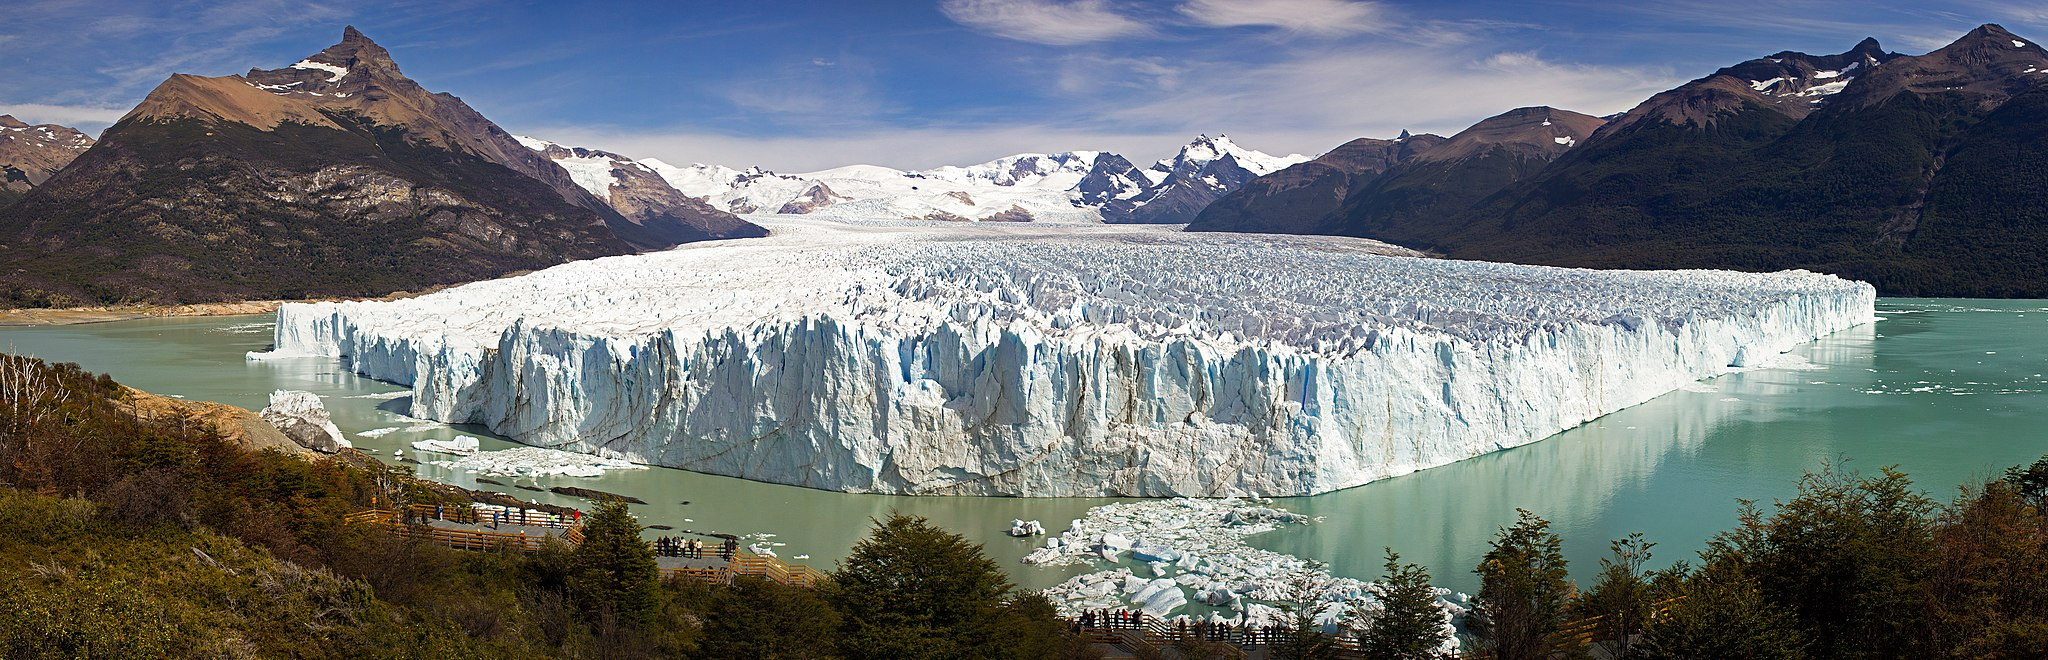
\includegraphics[width=.8\textwidth]{hyoga.jpg}
								\item コールタールも漏斗から\\流れ落ちる	
								
								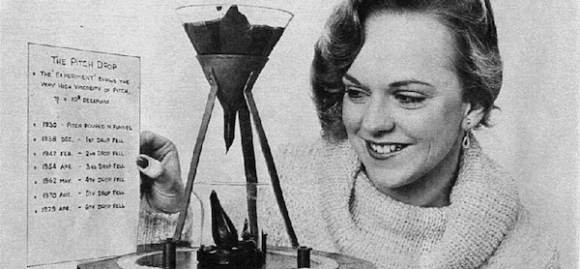
\includegraphics[width=.8\textwidth]{pitchdrop.png}
							\end{itemize}
						\end{itembox}
						\end{center}
					\end{minipage}
				\end{center}
				
			\qitem ガラス状態について
				\begin{center}
					\begin{minipage}{0.46\textwidth}
						\begin{itembox}[l]{ガラス状態}
							\begin{itemize}
								\item 液体からの冷却で、
								\item 常に\qbox{}するとは限らない。
								\begin{itemize}
									\item 非晶体:\qbox{}
									\item 流れない
									\item 例えば、\qbox{}等
								\end{itemize}
							\end{itemize}
						\end{itembox}
					\end{minipage}
					\begin{minipage}{0.4\textwidth}
						\begin{center}
						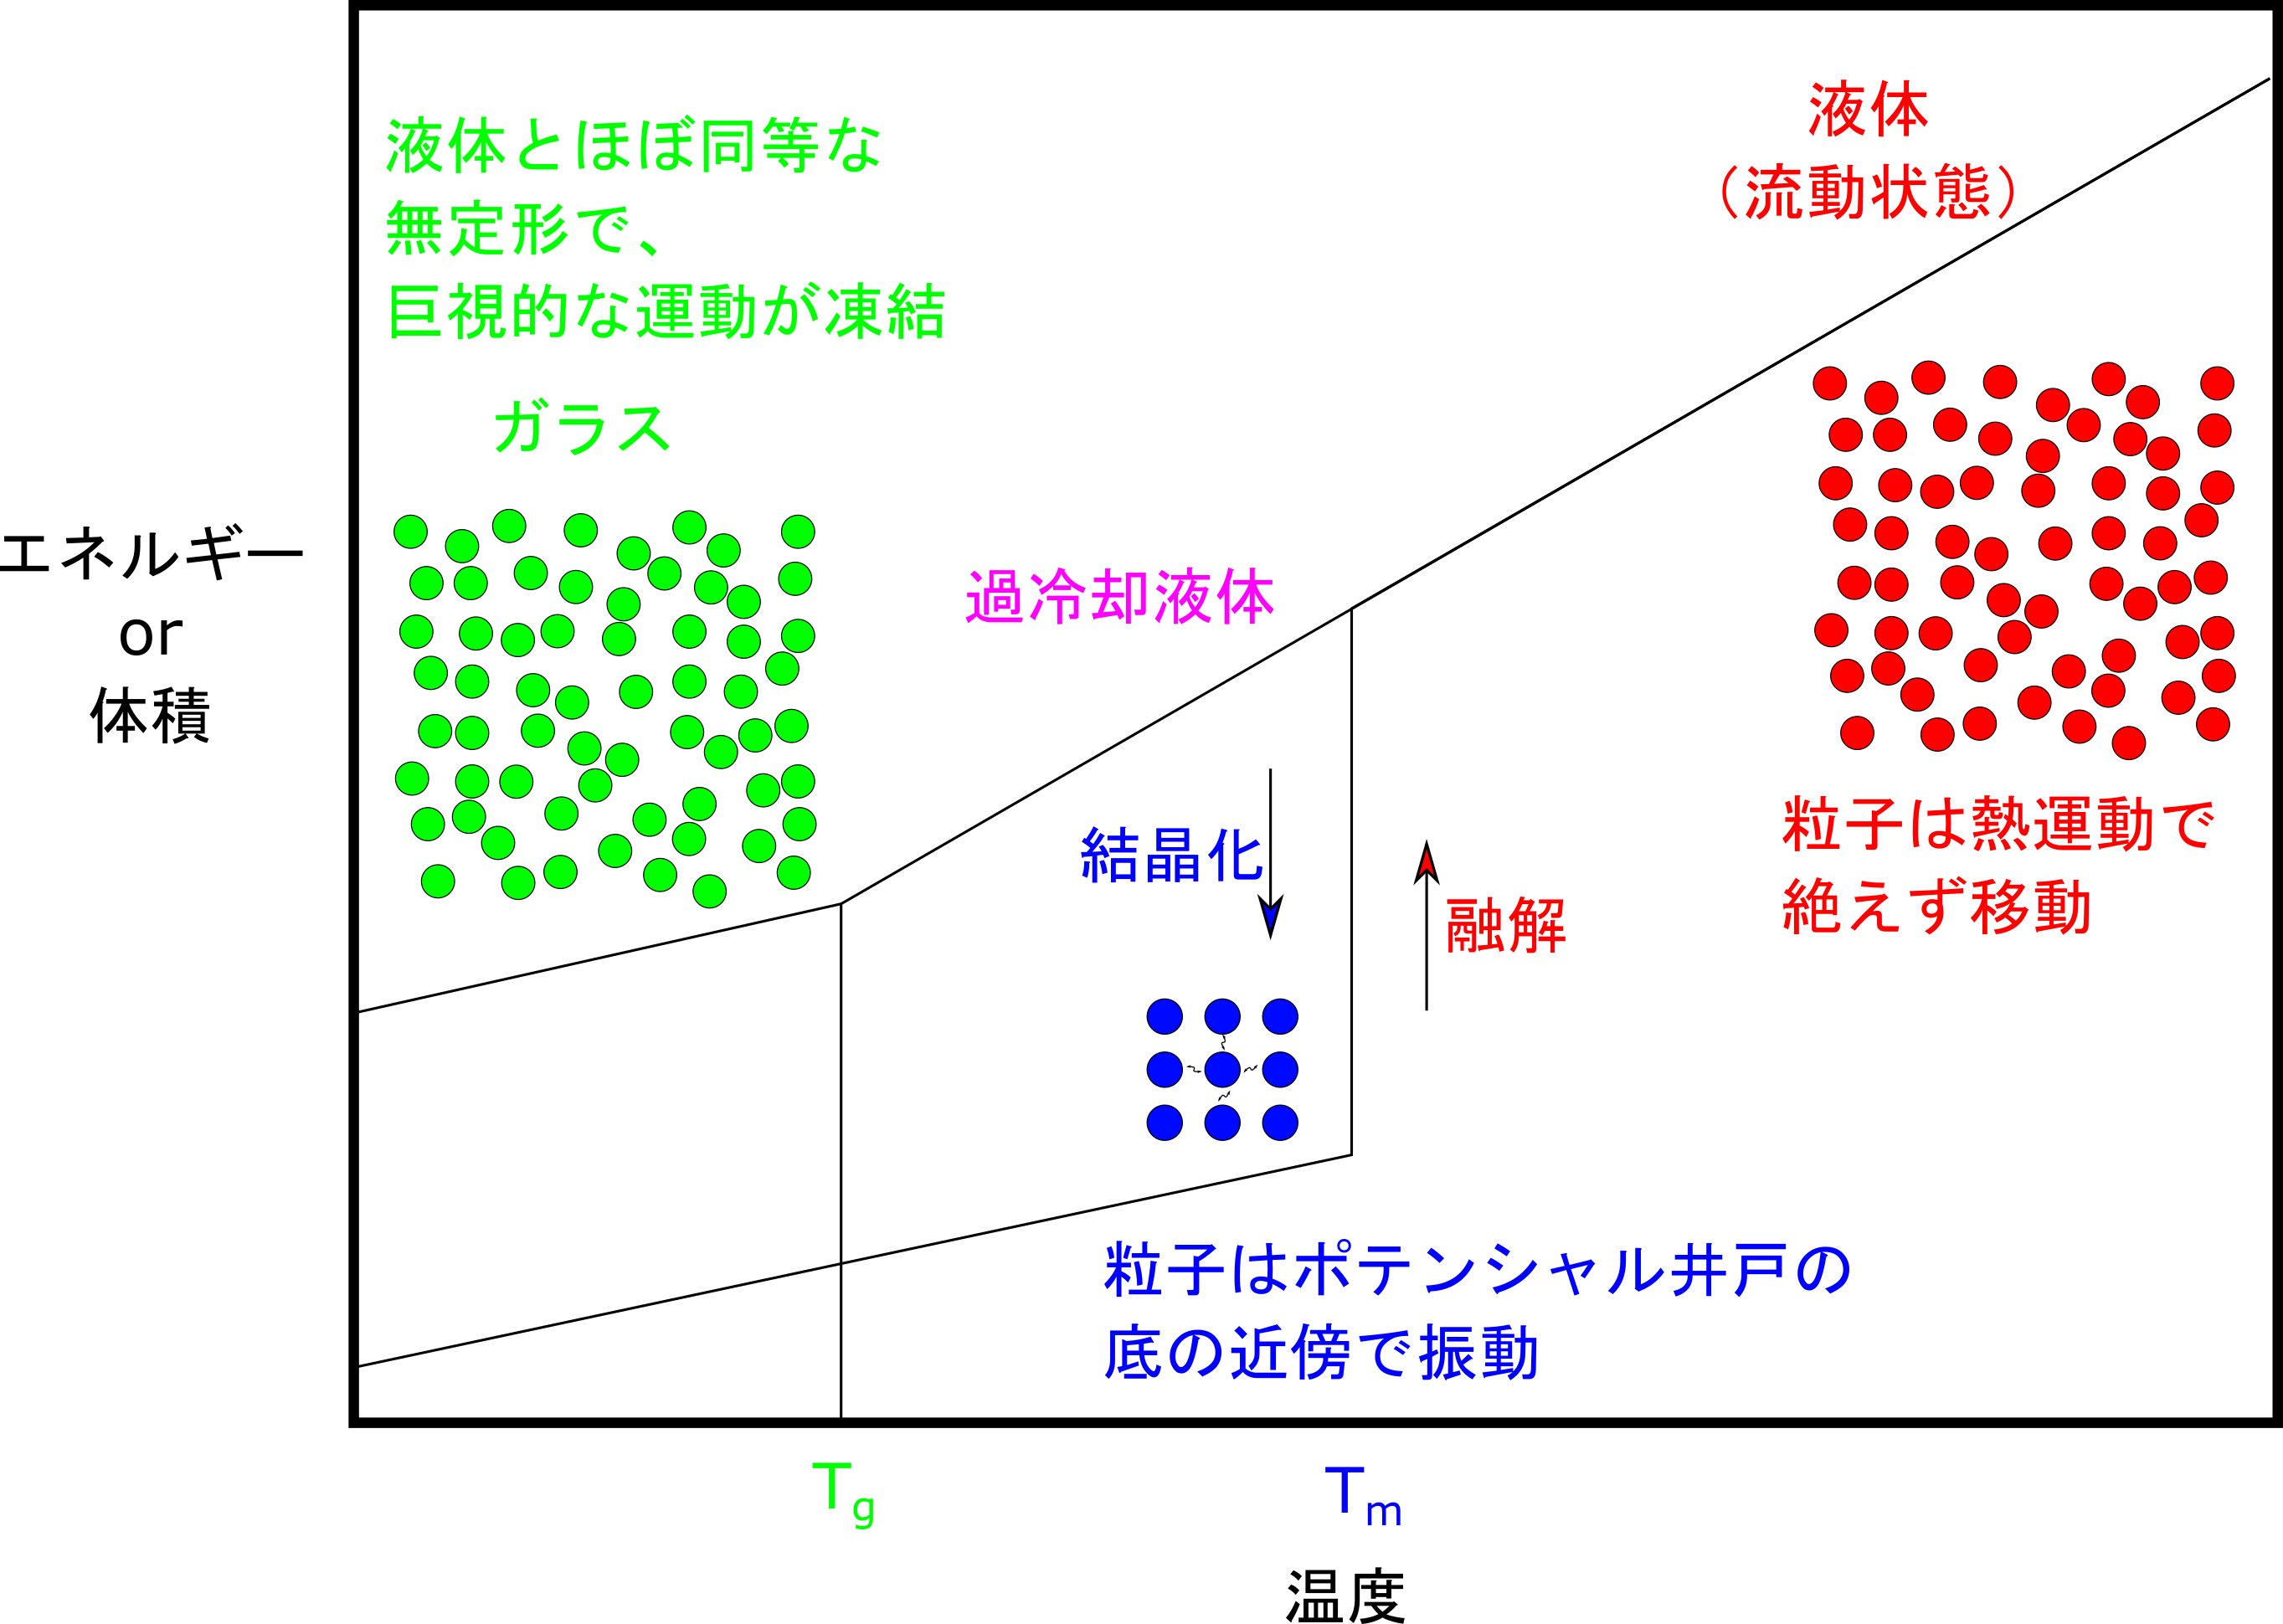
\includegraphics[width=\textwidth]{glass_trans.png}
						\end{center}
					\end{minipage}
				\end{center}
		\end{qlist2}

		\begin{itembox}[l]{選択肢}
			\begin{center}
				\begin{tabular}{lllll}
					1. 窓ガラス	&2. 再配置	&3. 液体的	&4. 最適化	&5. 速い変形\\
					6. アモルファス	&7. 結晶化		&8. 居心地が悪い	&9. 空いた場所
				\end{tabular}
			\end{center}
		\end{itembox}
\end{qlist}

\begin{itembox}[l]{解答}
    \begin{center} 
      \begin{tabular}{|c|c|c|c|c|c|c|c|c|} \hline
        (j) & (k) & (l) & (m) & (n) & (o) & (p) & (q) & (r)\\ \hline
         8  &  2 & 4 & 5 & 9 & 3 & 7 & 6 & 1 \\ \hline		
      \end{tabular}
    \end{center}
\end{itembox}


\begin{qlist}
	\qitem 「応力の起源」について、\qbox{(s)}から\qbox{(z)}までのカッコを埋めてください。
		\begin{qlist2}
			\qitem 結晶の応力の起源について
				\begin{center}
					\begin{minipage}{0.42\textwidth}
						\begin{itembox}[l]{マクロな変形の付与により}
							\begin{itemize}
								\item 固体内部でもミクロに変形
								\item マクロと相似に変形と単純化
								\item 粒子間で\qbox{}から変位
							\end{itemize}
						\end{itembox}
						\begin{center}
							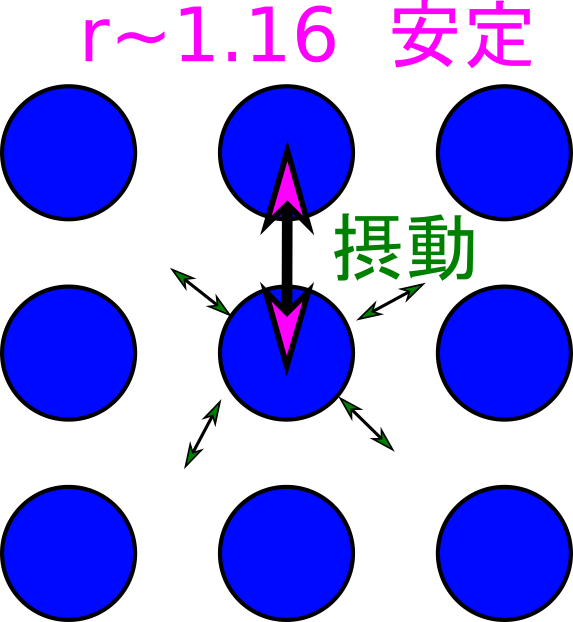
\includegraphics[width=.5\textwidth]{LJ_ryusi.png}
						\end{center}
					\end{minipage}
					\begin{minipage}{0.42\textwidth}
						\begin{itembox}[l]{ミクロに安定な位置から変位}
							\begin{itemize}
								\item 局所的には二体間で考えると、
								\begin{itemize}
									\item 接近した場合は、 $\Leftrightarrow$ 斥力
									\item 離反した場合は、 $\Leftrightarrow$ 引力
								\end{itemize}
								\item その\qbox{}として、マクロな応力が発生
							\end{itemize}
						\end{itembox}
						\begin{center}
							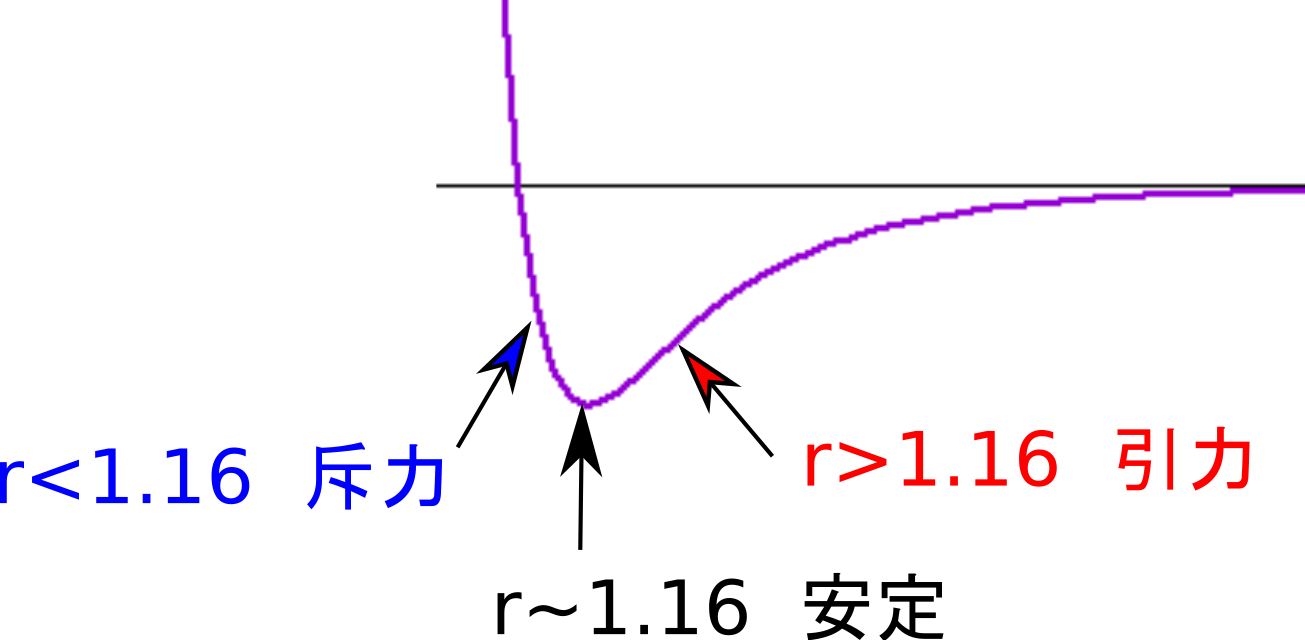
\includegraphics[width=\textwidth]{LJ_pos.png}
						\end{center}
					\end{minipage}
				\end{center}

			\qitem 固体と液体の違い
				\begin{itembox}[l]{固体と液体の違い}
					\begin{itemize}
						\item 固体では
						\begin{itemize}
							\item 単純な固体は一様に変形すると考えて、
							\item 生じる応力が一様で\qbox{}
						\end{itemize}
						\item 液体の場合
						\begin{itemize}
							\item 変形を止めれば、応力も\qbox{}すると考える。
							\item このとき、液体内部では、
							\begin{itemize}
								\item 粒子同士の相互作用が増加
								\item 粒子が\qbox{}すれば、増加分が消失
							\end{itemize}
						\end{itemize}
					\end{itemize}
				\end{itembox}
				
			\qitem 液体の応力について
				\begin{center}
					\begin{minipage}{0.42\textwidth}
						\begin{itembox}[l]{マクロな変形}
							\begin{itemize}
								\item マクロにせん断変形を付与
								\begin{itemize}
									\item ミクロにも粒子近傍が変形
								\end{itemize}
								\item 一粒子に着目すると、
								\begin{itemize}
									\item ポテンシャル場が変化
									\item 局所的に「\qbox{}」
								\end{itemize}
							\end{itemize}
						\end{itembox}
						\begin{center}
							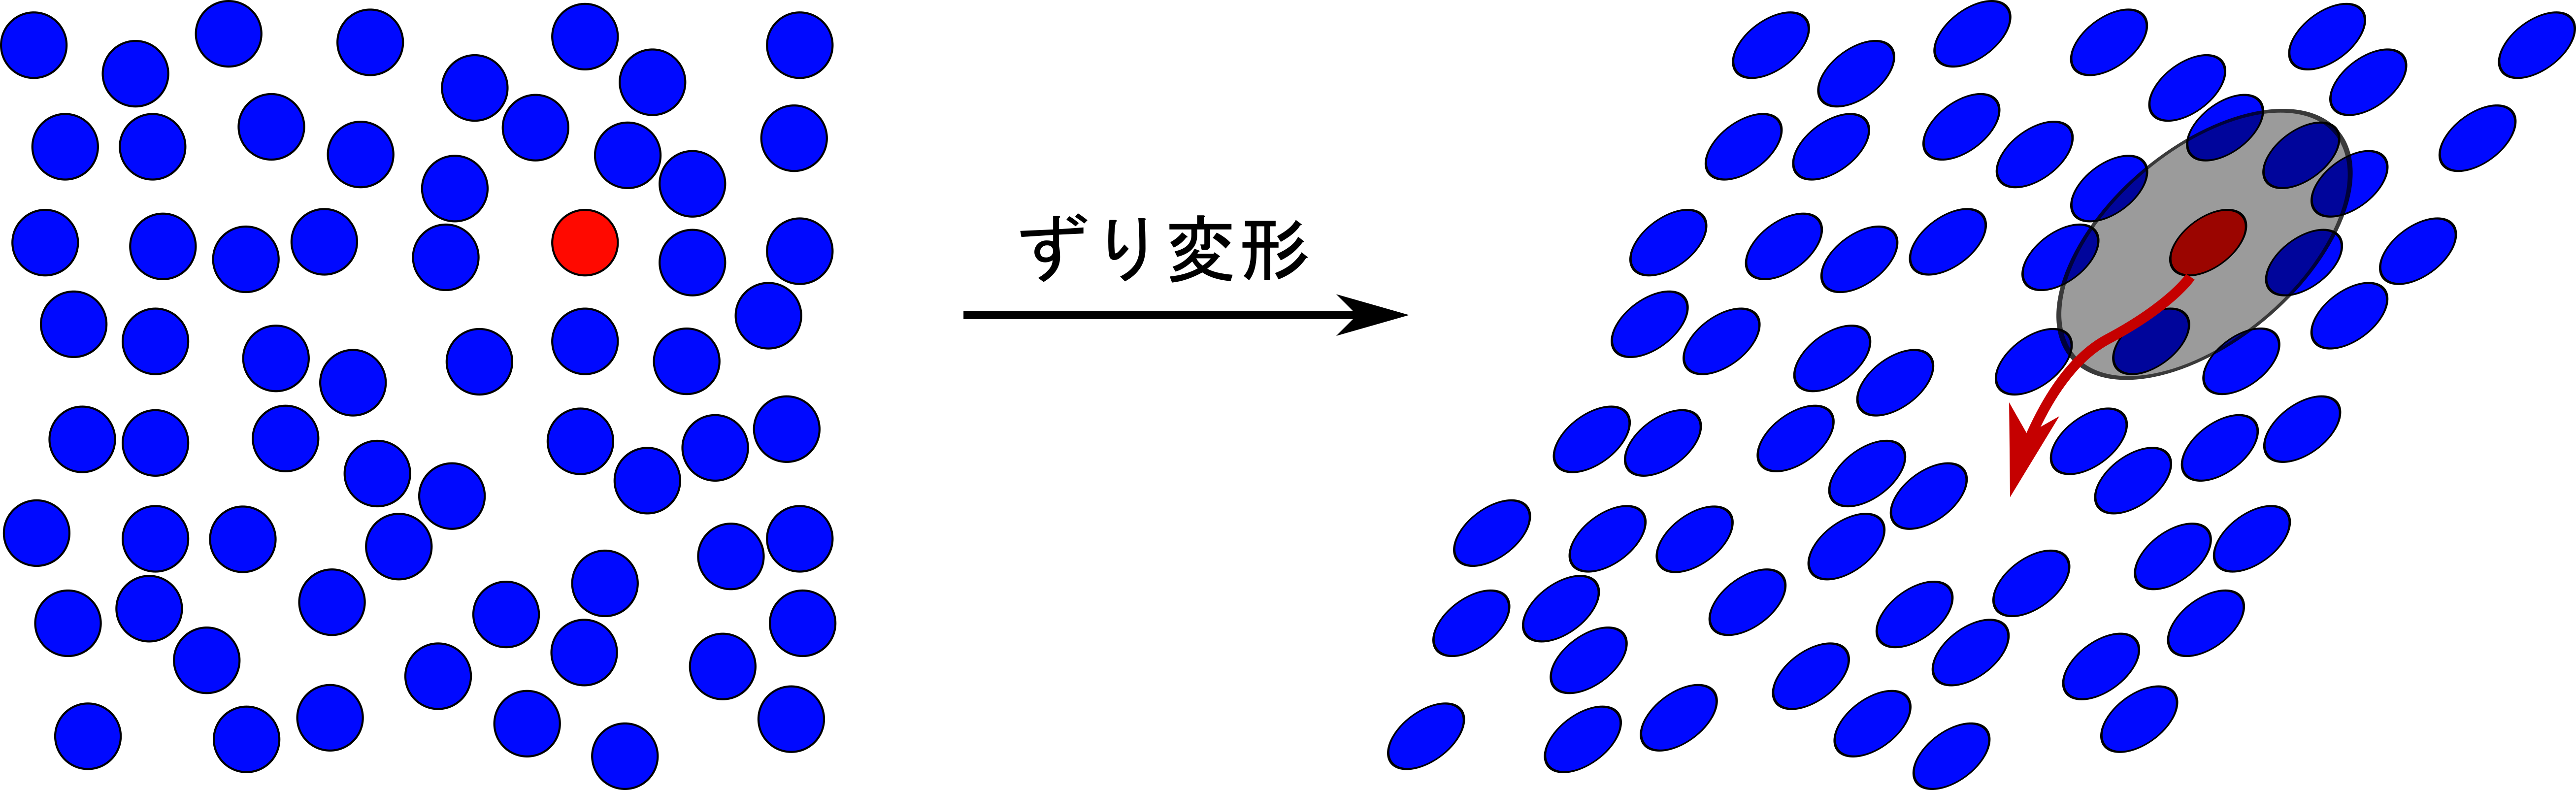
\includegraphics[width=.9\textwidth]{liquid_flow.png}
						\end{center}
					\end{minipage}
					\begin{minipage}{0.42\textwidth}
						\begin{itembox}[l]{ミクロな応力から流動へ}
							\begin{itemize}
								\item 「歪んだかご」の結果、
								\begin{itemize}
									\item 粒子の\qbox{}が悪化
									\item 局所的な応力が発現
									\item 積分値としてマクロな応力
								\end{itemize}
								\item 「歪んだかご」からの脱出
								\begin{itemize}
									\item ミクロな応力が消失
								\end{itemize}
								\item マクロにも\qbox{}
								\begin{itemize}
									\item マクロな応力も消失
								\end{itemize}
							\end{itemize}
						\end{itembox}
					\end{minipage}
				\end{center}
		\end{qlist2}

		\begin{itembox}[l]{選択肢}
			\begin{center}
				\begin{tabular}{lllll}
					1. 移動	&2. 居心地 	&3. 消失	&4. 積分値	&5. 持続的\\
					6. 流動	&7. 歪んだかご &8. 安定位置
				\end{tabular}
			\end{center}
		\end{itembox}
\end{qlist}

\begin{itembox}[l]{解答}
    \begin{center} 
      \begin{tabular}{|c|c|c|c|c|c|c|c|} \hline
        (s) & (t) & (u) & (v) & (w) & (x) & (y) & (z) \\ \hline
        8 & 4 & 5 & 3 & 1 & 7 & 2 & 6 \\ \hline		
      \end{tabular}
    \end{center}
\end{itembox}

\clearpage

\question{演習問題 3}
説明文中の言葉を使って数行程度の簡単な記述で構いませんので、以下の自由記述問題を考えてみてください。
\begin{qlist}
\qitem この章では、物理化学として物質を見直すという観点で、固体と液体の違いについてミクロなイメージの説明を行いました。

レオロジーという学問においては、流れるということが最も重要な現象となりますので、
文中の言葉をそのまま使って結構ですから、ご自分なりの「流れるとはどういう現象なのか」ということを書いてみてください。
\end{qlist}

\begin{itembox}[l]{解答例}
    流れるという現象は、マクロに与えた変形等の刺激に対して、液体がその形を変えることによって、与えられた刺激をなかったことにしていく過程と考えることができる。
	なお、変形を与えている間は、その変形速度に比例する形で移動(流れ)を止めようとする応力が発生する。

	この現象をミクロに見ると、物質の内部で粒子の居心地が悪くなった際に、それを改善するためにミクロな物質の移動が生じていると考えることが出来る。
\end{itembox}

\clearpage

\end{document}
\clearpage

\end{document}